% !TEX TS-program = xelatex
% !TEX encoding = UTF-8 Unicode
% !Mode:: "TeX:UTF-8"

\documentclass{resume}
\usepackage{stys/zh_CN-Adobefonts_external} % Simplified Chinese Support using external fonts (./fonts/zh_CN-Adobe/)
% \usepackage{stys/NotoSansSC_external}
% \usepackage{stys/NotoSerifCJKsc_external}
% \usepackage{stys/zh_CN-Adobefonts_internal} % Simplified Chinese Support using system fonts
\usepackage{stys/linespacing_fix} % disable extra space before next section
\usepackage{bookmark}
\usepackage{cite}
\usepackage{graphicx} % for header_with_photo. avatar
\usepackage{tabularray} % for header_with_photo

\newif\ifacademic
\academictrue % 教职/学术版（完整内容）。业界版见 resume-zh_CN.tex

\begin{document}
\pagenumbering{gobble} % suppress displaying page number

\settitlelinestyle{default} % partialbg, fullbg
% \settitlelinestyle{partialbg}
% \settitlelinestyle{fullbg}

% 需要入口文件启用 graphicx 与 tabularray 两个宏包
% 照片占位图为 images/avatar.jpg —— 换成本人证件照即可，无需改本文件
\begin{tblr}{
    width = \linewidth,
    colspec = {Q[l,2.35cm]X[c]Q[r,2.35cm]},
    % rows = {abovesep=0pt, belowsep=0pt},
    columns = {colsep=2pt},
    row{1} = {ht=2.4em, font=\Huge},
    row{3} = {ht=2em, abovesep=0pt},
  }
  & 王虎林 & \SetCell[r=3]{f} 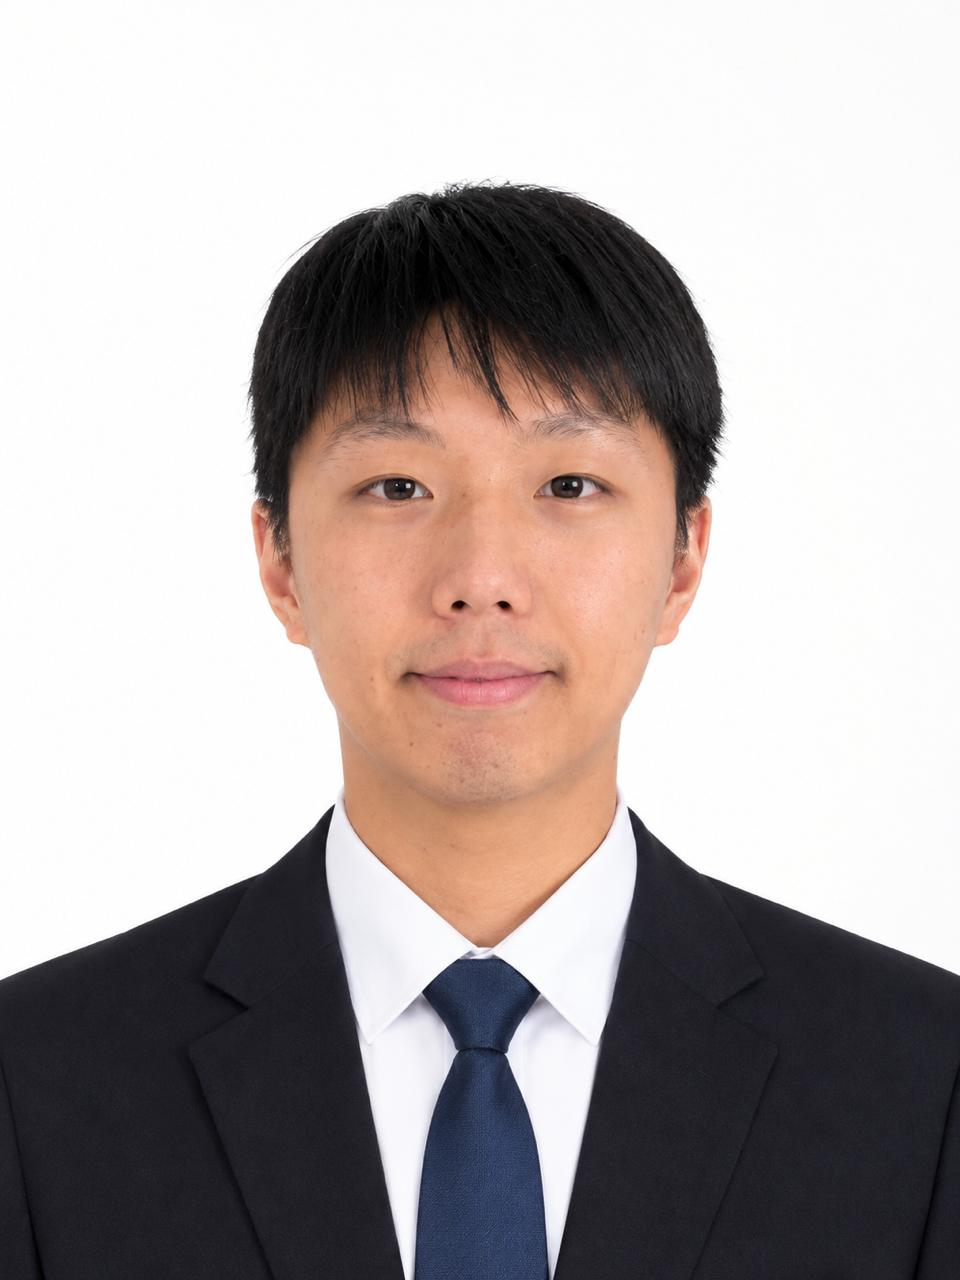
\includegraphics[width=0.9in]{images/avatar} \\
  & \identity{政治面貌：群众}\dotSep \hometown{籍贯：辽宁}\dotSep \calendar{1998.5.30} &  \\
  & \github[DeviRule]{https://github.com/DeviRule}\dotSep
    % \linkedin[hulin-wang]{https://www.linkedin.com/in/hulin-wang-4ab350164/}\dotSep
    % \homepage[hulinwang.me]{https://www.hulinwang.me/} \dotSep 
     \phone{13756007928}\dotSep \email{hwang551@asu.edu}
\\
\end{tblr}

% \name{王虎林}

\basicInfo{
  \identity{博士研究生在读 · 预计 2027.12 毕业}\dotSep
  \email{hwang551@asu.edu}
  % TODO: 补充电话后取消注释 \dotSep\phone{000-0000-0000}
}

\basicInfo{
  \github[DeviRule]{https://github.com/DeviRule}\dotSep
  \linkedin[hulin-wang]{https://www.linkedin.com/in/hulin-wang-4ab350164/}\dotSep
  \homepage[hulinwang.me]{https://www.hulinwang.me/}\dotSep
  \hometown{美国 亚利桑那州 坦佩}
}
 % 不带照片的版本
% ============================================================================
%  内容单一来源。两版内容深度相同，差异仅 3 处，由 \ifacademic 控制：
%    1. USC / UC Davis 的 GPA —— 仅教职版显示
%    2. 荣誉与奖学金 —— 业界版合并一节，教职版拆「荣誉奖项」「奖学金」两节
%    3. LitePoint 本科实习 —— 仅业界版显示
%  开关在入口文件里设置：resume-zh_CN.tex（业界）/ resume-zh_CN-academic.tex（教职）
% ============================================================================

\sectionTitle{求职意向}{\faiconsixbf{bullseye}}
\begin{onehalfspacing}
\ifacademic
\normalline{\textbf{目标岗位}：助理教授（tenure-track）\dotSep 高校/研究院研究员}
\normalline{\textbf{研究方向}：软件与系统安全 \dotSep 漏洞挖掘与自动修复 \dotSep 人工智能安全}
\else
\normalline{\textbf{目标岗位}：软件安全研究员 \dotSep 安全工程师 \dotSep 人工智能安全研究员}
\normalline{\textbf{关注领域}：漏洞挖掘与自动修复 \dotSep 模糊测试 \dotSep 大模型与智能体安全}
\fi
\normalline{\textbf{期望城市}：深圳 \dotSep \textbf{可到岗时间}：2028.01（预计 2027 年秋季毕业）}
\end{onehalfspacing}

\sectionTitle{教育背景}{\faiconsixbf{graduation-cap}}
\datedsubsection{\texthl{亚利桑那州立大学（Arizona State University）} / \textit{计算机科学} / \textit{博士} / GPA 4.0/4.0}{2022.08 -- 2027.12}
\subline{SEFCOM 安全实验室 \dotSep 导师：\textbf{Tiffany Bao、Fish Wang} \dotSep 计算机安全方向 \textbf{CSRankings 全美前五}}
\datedsubsection{\texthl{南加州大学（University of Southern California）} / \textit{计算机科学} / \textit{硕士} / GPA 3.6/4.0}{2020.08 -- 2022.05}
\datedsubsection{\texthl{加州大学戴维斯分校（UC Davis）} / \textit{计算机科学} / \textit{学士}\ / GPA 3.7/4.0}{2016.09 -- 2020.06}

\sectionTitle{工作与研究经历}{\faiconsixbf{building-user}}

\datedsubsection{\textbf{亚马逊（Amazon）}\ 美国·纽约}{2026.05 -- 2026.08}
\role{应用科学家实习生（Applied Scientist Intern）}{}
\normalline{\textbf{面向静态分析规则开发的多智能体告警研判系统}}
\begin{itemize}
\item 自动判断生产环境里的静态分析告警是否有效，把单条规则的验证周期从 10--15 天压到 2--3 天；判断准确率 90\%，平均每条告警处理耗时 4 分钟，成本 \$0.50
\item 用 Strands Agent SDK 搭了一套多智能体工作流，先做告警摘要，再收集相关代码，最后验证；用同一个模型时，评测得分比 Claude Code 高 14 分
\item 支持两套内部静态分析器的全部 47 条规则，覆盖 Python、Java、JavaScript；不用针对某条规则或某种语言单独调参
\item 从过去一年的生产告警分析记录里整理了 600+ 条测试样本，覆盖所有规则；运行五次下来，判断结果一致率 95\%
\end{itemize}
\datedsubsection{\textbf{亚利桑那州立大学 SEFCOM 安全实验室}\ 美国·坦佩}{2022.08 -- 至今}
\role{博士研究生}{}
\normalline{\textbf{根因驱动的漏洞修复（Root-Cause-Driven Patching）}}
\begin{itemize}
\item 设计了一套两阶段自动修复漏洞的流程：先用静态分析结合程序运行信息，定位漏洞可能的根因，能找出 CodeQL 这类纯静态工具漏掉的跨位置缺陷和间接调用
\item 把定位结果交给一个轻量修复 Agent，并给它仓库搜索和文件编辑工具，让它理解相关代码后生成补丁
\item 收集并整理 178 个 C/C++ 漏洞，逐个人工标注补丁质量，用来对比不同 Agent 的修复效果
\item 请三位专家评审，按多数意见确定最终结果；相比 ChatGPT Codex 等通用编码 Agent，补丁质量提升了 20%
\end{itemize}
\normalline{\textbf{无人机固件安全与信息物理漏洞挖掘}}
\normalline{美国国防高级研究计划局资助项目FIRE， 资助800万美金}
\begin{itemize}
\item 主导无人机飞控（ArduPilot 及某商用衍生版本）的 sim-to-real 漏洞测试流水线：先通过固件指纹判断机型和版本，在 PX4 / Gazebo SITL 里重建目标环境，再对配置参数、指令和物理状态做策略引导模糊测试（PGFuzz）
\item 在真实机架上复现了 2 组已知的策略违例输入集，说明降保真度仿真不用数字孪生也能反映真实硬件行为
\item 从零搭起 ARM Cortex-M 裸机固件重宿主（rehosting）能力：用 flash dump 配合自定义链接脚本重建 ELF 镜像，再通过二进制修补绕过架构检查、处理未建模的 MMIO 读取，让固件能在 QEMU 下跑起来；同时加入 GDB 插桩做在线内存检查，最后作为团队动态分析基座交付
\item 从剥离符号的固件里恢复符号：推断原始工具链，交叉编译匹配的开源库，再在 IDA Pro / Ghidra 里做 FLIRT 签名匹配
\end{itemize}
\normalline{\textbf{LLM辅助的模糊测试研究}}
\begin{itemize}
\item 设计并实现了一条 LLM 辅助的源码修补 + AFL++ 模糊测试（fuzzing）流水线，用来挖成熟代码库里那些被更容易触发的崩溃掩盖住的遮蔽缺陷（occluded bugs）
\item 把流程串成自动闭环：崩溃聚类、根因提示 → LLM 改源码 → 重新构建 → 再跑 fuzz；中间用定向回归测试确认修复没问题。误报率从 90\% 降到 30\%，最后产出详细漏洞报告和 PoC 测试用例
\item 在 Objdump、FFmpeg、GPAC 等项目上，单目标发现 20+ 个独立遮蔽漏洞，包括 Use-After-Free、堆/栈溢出和段错误，都用 ASan/MSan 及定向回归测试验证过
\end{itemize}

\datedsubsection{\textbf{Team Shellphish / 人工智能网络安全挑战赛（AIxCC）}\ 美国·坦佩}{2023.08 -- 2025.08}
\role{漏洞修复组件负责人（Patching Component Lead）}{}
\normalline{美国国防高级研究计划局人工智能网络安全挑战赛（AIxCC）：面向真实开源和关键基建软件的自动化漏洞发现与修复的全球竞赛，团队获\textbf{第五名}，团队奖金 \textbf{200 万美元}}
\normalline{\textbf{安全漏洞修复智能体}}
\begin{itemize}
\item 负责搭建多智能体漏洞修复系统，让系统能自主判断、生成补丁并验证，把分散在不同服务里的组件串成完整流程
\item 给智能体加了反馈闭环：跑 fuzzing、复现崩溃样本、跑确定性回归测试来检查补丁；只有真正修掉漏洞（不是只让崩溃消失）且不影响原有功能的补丁才会通过。最终计分轮补丁正确率 $>$95%
\item 在 curl、NGINX、Apache ZooKeeper 等大型开源项目上分析并修复了 30+ 个 C/Java 漏洞，涉及缓冲区溢出（Buffer Overflow）、释放后重用（Use After Free）、命令注入（Command Injection）、路径穿越（Path Traversal）等类型
\end{itemize}

\normalline{\textbf{漏洞验证用例（PoC）生成智能体}}
\begin{itemize}
\item 开发了一套多智能体系统，把静态分析结果和上下文信息结合起来，生成能定向触发崩溃的测试用例
\item 先做基于可达性的程序切片，给智能体划出更聚焦的代码路径来生成输入，再用覆盖率引导搜索绕过阻断逻辑
\item 平均 5 分钟就能生成触发崩溃的测试用例；在 ZooKeeper、Tika、jsoup 等开源项目（1 万–10 万行代码）里发现 10 个漏洞，其中 5 个是 Jazzer 连续跑 8 小时都没发现的
\end{itemize}

\datedsubsection{\textbf{南加州大学 ITS 治理、风险与合规（GRC）团队}\ 美国·洛杉矶}{2021.10 -- 2022.05}
\role{学生研究员（Student Researcher）}
\normalline{\textbf{校园 IT 风险评估与漏洞治理平台}}
\begin{itemize}
  \item 设计并上线 4 项风险评估指标及配套监控系统，评估校级基础设施的安全态势，以 Python 构建可扩展的分析方案实现风险实时量化
  \item 构建分析框架度量并优化 BigFix 补丁分发系统的效率，向校方管理层汇报技术结论，将复杂数据转化为可执行的决策依据
  \item 搭建自动化监控与告警基础设施，整合 SentinelOne 等多源数据计算风险指标，向安全运营团队实时推送告警
\end{itemize}

\ifacademic\else
\datedsubsection{\textbf{LitePoint}\ 美国·圣何塞}{2019.06 -- 2019.09}
\role{软件工程实习生（Software Engineer Intern）}{}
\normalline{\textbf{制造数据 ETL 入库与查询优化}}
\begin{itemize}
\item 以 Python 构建抽取—转换—加载（ETL）系统，将原始制造数据自动写入 Microsoft SQL Server 数据库
\item 实现后端流水线：从指定服务器自动拉取 10GB 新增 CSV 文件，完成数据清洗并以并行加载流在 2 分钟内入库
\item 通过为高频表建立索引、使用优化器提示（optimizer hints）、重构陈旧 SQL 语句，将查询性能提升 \textbf{500\%}
\end{itemize}
\fi

\sectionTitle{论文发表}{\faiconsixbf{book}}
\begin{onehalfspacing}
\datedline{\textbf{Root-Cause-Driven Automated Vulnerability Repair} / \textit{第一作者} / \textit{在投}}{2026.04}
\datedline{\textbf{SeedSmith: LLM-Driven Seed Synthesis for Directed Fuzzing} / \textit{在投}}{2026.04}
\datedline{\textbf{BuildBench: Benchmarking LLM Agents on Compiling Real-World Open-Source Software} / \textit{TMLR 2026}}{2026.04}
\datedline{\textbf{AIJon: Automated Generation of Annotations for Fuzzing} / \textit{arXiv}}{2026.02}
\datedline{\textbf{FedNLP: A Research Platform for Federated Learning in NLP} / \textit{NAACL 2022 Findings (CCF B)}}{2022.04}
\end{onehalfspacing}
\ifacademic
\sectionTitle{荣誉奖项}{\faiconsixbf{award}}
\begin{onehalfspacing}
\datedline{DARPA AI 网络挑战赛（AIxCC）\space / \textit{全球第五名}}{2025.08}
\datedline{DEF CON CTF 全球总决赛（Team Shellphish）\space / \textit{第 11 名}}{2025.08}
\datedline{ACM CCS 2024 杰出论文成果评估奖（Distinguished Artifact Reviewer Award）}{2024.10}
\datedline{DEF CON CTF 全球总决赛（Team Shellphish）\space / \textit{第 11 名}}{2023.08}
\end{onehalfspacing}

\sectionTitle{奖学金}{\faiconsix{google-scholar}}
\begin{onehalfspacing}
\datedline{亚利桑那州立大学 SCAI 博士研究生奖学金（SCAI Doctoral Fellowship）}{2022.08}
\datedline{亚利桑那州立大学 Fulton Fellowship}{2022.08}
\datedline{PLDI 2022 PLMW Scholarship}{2022.06}
\end{onehalfspacing}
\else
\sectionTitle{荣誉与奖学金}{\faiconsixbf{award}}
\begin{onehalfspacing}
\datedline{DARPA 人工智能网络安全挑战赛（AIxCC）\space / \textit{全球第五名}}{2025.08}
\datedline{DEF CON CTF 全球总决赛（Team Shellphish）\space / \textit{第 11 名}}{2025.08}
\datedline{ACM CCS 2024 杰出论文成果评估奖（Distinguished Artifact Reviewer Award）}{2024.10}
\datedline{DEF CON CTF 全球总决赛（Team Shellphish）\space / \textit{第 11 名}}{2023.08}
\datedline{亚利桑那州立大学 SCAI 博士研究生奖学金（SCAI Doctoral Fellowship）}{2022.08}
\datedline{亚利桑那州立大学 Fulton Fellowship}{2022.08}
\datedline{PLDI 2022 PLMW Scholarship}{2022.06}
\end{onehalfspacing}
\fi

\sectionTitle{学术服务}{\faiconsixbf{clipboard-check}}
\begin{onehalfspacing}
\normalline{\textbf{期刊审稿}：IEEE TDSC（CCF A）、ACM TIST（CCF B，外部审稿人）}
\normalline{\textbf{论文成果评估（Artifact Evaluation）委员}：IEEE S\&P 2026、ACM CCS 2024（均为 CCF A）}
\end{onehalfspacing}

\ifacademic
\sectionTitle{教学经历}{\faiconsixbf{chalkboard-user}}
\begin{onehalfspacing}
\datedline{亚利桑那州立大学\space CSE 365《网络安全导论》\space 助教（Teaching Assistant）}{2023.08 -- 2023.12}
\end{onehalfspacing}
\fi

\sectionTitle{专业技能}{\faiconsixbf{gears}}
\begin{onehalfspacing}
\normalline{\textbf{编程语言}：C/C++、Python、Java、OCaml、TypeScript、SQL}
\normalline{\textbf{安全与逆向}：AFL++、Jazzer、PGFuzz、CodeQL、IDA Pro、Ghidra、angr、QEMU、GDB}
\normalline{\textbf{大模型与智能体}：OpenAI Agents SDK、LangChain、PyTorch、Hugging Face Transformers}
\normalline{\textbf{系统、数据库与嵌入式}：Docker、Kubernetes、Microsoft SQL Server、SQLite、Neo4j、PX4 / Gazebo SITL}
\end{onehalfspacing}


%% Reference
% \newpage
% \bibliographystyle{cites/IEEETran}
% \bibliography{cites/mycite}
\end{document}
